\documentclass[times, utf8, zavrsni]{fer}
\usepackage{booktabs}
\usepackage{color}
\usepackage{listings}
\usepackage{minted}
\usepackage{siunitx}

\setminted{tabsize=3,linenos,breaklines,breakanywhere,fontsize=\tiny}

\graphicspath{{C:/Users/Nikola/Programming/CUBE_workspace/FERSAT_PDH/brzistart/slike/}}

\begin{document}

% TODO: Navedite broj rada.
\thesisnumber{2021-72}

% TODO: Navedite naslov rada.
\title{Programska potpora za upravljanje kamerom na CubeSat nanosatelitu}

% TODO: Navedite vaše ime i prezime.
\author{Nikola Gudan}

\maketitle

% Ispis stranice s napomenom o umetanju izvornika rada. Uklonite naredbu \izvornik ako želite izbaciti tu stranicu.
\izvornik

% Dodavanje zahvale ili prazne stranice. Ako ne želite dodati zahvalu, naredbu ostavite radi prazne stranice.
\zahvala{}

\tableofcontents

\chapter{Uvod}
Uvod rada. Nakon uvoda dolaze poglavlja u kojima se obrađuje tema.

\chapter{I\textsuperscript{2}C sučelje mikrokontrolera STM32L471VGT6}
Za konfiguraciju kamere Arducam 5MP Mini Plus  PDH računalo koristi I\textsuperscript{2}C komunikaciju. S obzirom na to da se za razvoj programske potpore PDH računala koriste \textit{Low-Layer} biblioteke, potrebno je razumijevanje načina rada I\textsuperscript{2}C periferije odabranog mikrokontrolera kako bi se ispravno implementirali upravljački programi. U nastavku slijedi općenit opis I\textsuperscript{2}C komunikacije kao i njena implementacija na STM32L471VGT6 mikrokontroleru.

\section{I\textsuperscript{2}C protokol}
I\textsuperscript{2}C (\textit{Inter-Integrated Circuit}) je jednostavna dvosmjerna sinkrona serijska sabirnica razvijena od strane \textit{Philips Semiconductors} (sada \textit{NXP Semiconductors}) 1982. godine. Koristi dvije linije:
\begin{itemize}
\item serijska podatkovna linija (SDA, \textit{Serial Data Line}),
\item serijska taktna linija (SCL, \textit{Serial Clock Line}),
\end{itemize}
obje linije su pritegnute na visoku logičku razinu preko \textit{pull-up} otpornika. Moguće brzine prijenosa su:
\begin{itemize}
\item do 100 \si{kbit/s} u \textit{Standard-mode} načinu rada, 
\item do 400 \si{kbit/s} u \textit{Fast-mode} načinu rada,
\item do 1 \si{Mbit/s} u \textit{Fast-mode Plus} načinu rada,
\item do 3.4 \si{Mbit/s} u \textit{High-speed} načinu rada.
\end{itemize}
Navedene brzine se koriste kod dvosmjernog prijenosa, a moguća je i brzina do 5 \si{Mbit/s} u jednosmjernom prijenosu. Više uređaja se može spojiti na jednu sabirnicu, a svaki uređaje je prepoznatljiv po svojoj jedinstvenoj adresi i može se ponašati kao prijamnik ili odašiljač, ovisno o funkciji uređaja. Protokol najčešće, a tako i u ovom slučaju, koristi 7-bitno adresiranje, a moguće je i korištenje 10-bitnog adresiranja. Uz prijamnike i odašiljače uređaj također može biti upravljač ili meta tijekom prijenosa podataka. Upravljač je uređaj koji inicijalizira prijenos podataka na sabirnici i generira signal takta kako bi omogućio prijenos. U tom trenutku, bilo koji uređaj koji je adresiran smatra se metom.

Na I\textsuperscript{2}C sabirnicu se također može spojiti više upravljača, a primjer jednog takvog spoja sa dva mikrokontrolera je dan na sljedećoj slici.

\begin{figure}[htp]
\centering
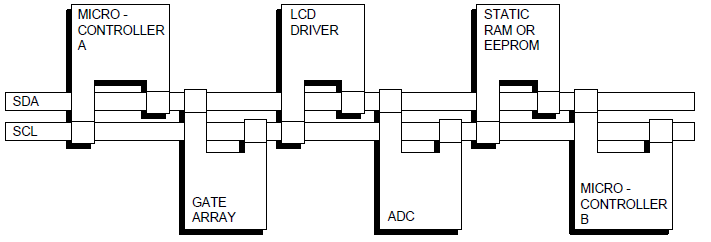
\includegraphics[width=\textwidth]{i2c_primjer_1.PNG}
\caption{Primjer I\textsuperscript{2}C sabirnice sa spojena dva mikrokontrolera}
\label{fig:i2c_primjer_1}
\end{figure}

\chapter{Zaključak}
Zaključak.

\bibliography{literatura}
\bibliographystyle{fer}

\begin{sazetak}
Sažetak na hrvatskom jeziku.

\kljucnerijeci{Ključne riječi, odvojene zarezima.}
\end{sazetak}

% TODO: Navedite naslov na engleskom jeziku.
\engtitle{Software for Camera Control on CubeSat Nanosatellite}
\begin{abstract}
Abstract.

\keywords{Keywords.}
\end{abstract}

\end{document}
